% This file was created by tikzplotlib v0.9.8.
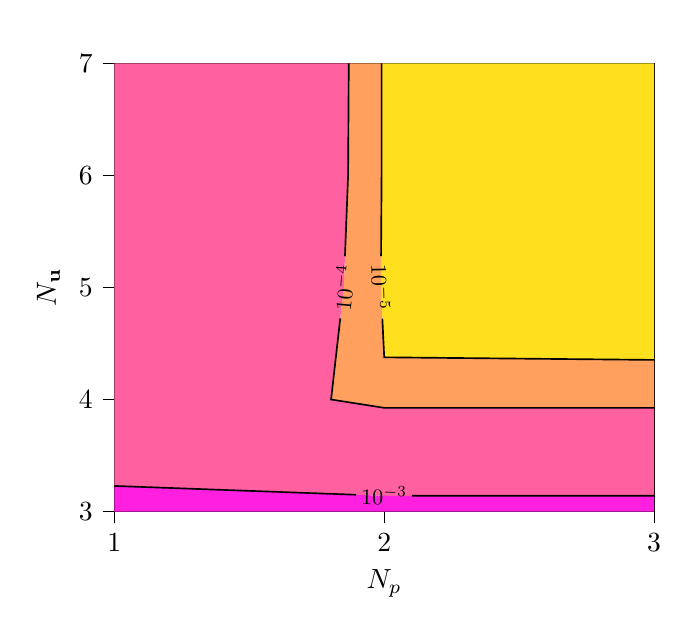
\begin{tikzpicture}

\definecolor{color0}{rgb}{1,0.87843137254902,0.12156862745098}
\definecolor{color1}{rgb}{1,0.627450980392157,0.372549019607843}
\definecolor{color2}{rgb}{1,0.376470588235294,0.623529411764706}
\definecolor{color3}{rgb}{1,0.125490196078431,0.874509803921569}

\begin{axis}[
tick align=outside,
tick pos=left,
%title={Relative Error in Velocity \(\displaystyle \mathbf{u}\) - Max},
title={$\relErrorVelocity$},
x grid style={white!69.0196078431373!black},
xlabel={\(\displaystyle N_p\)},
xmin=1, xmax=3,
xtick style={color=black},
xtick={1,2,3},
xticklabels={\(\displaystyle 1\),\(\displaystyle 2\),\(\displaystyle 3\)},
y grid style={white!69.0196078431373!black},
ylabel={\(\displaystyle N_{\mathbf{u}}\)},
ymin=3, ymax=7,
ytick style={color=black},
ytick={3,4,5,6,7},
yticklabels={
  \(\displaystyle 3\),
  \(\displaystyle 4\),
  \(\displaystyle 5\),
  \(\displaystyle 6\),
  \(\displaystyle 7\)
}
]
\addplot [draw=none, fill=color0]
table{%
x  y
2 4.37650891394412
3 4.35330770412385
3 5
3 6
3 7
2 7
1.99040991259345 7
1.9903127173998 6
1.98760845108052 5
2 4.37650891394412
};
\addplot [draw=none, fill=color1]
table{%
x  y
2 3.92579367910137
3 3.92540471448223
3 4
3 4.35330770412385
2 4.37650891394412
1.98760845108052 5
1.9903127173998 6
1.99040991259345 7
1.86869012295147 7
1.86619036626405 6
1.85013870710813 5
1.80309130655496 4
2 3.92579367910137
};
\addplot [draw=none, fill=color2]
table{%
x  y
2 3.14101234840689
3 3.14081265825156
3 3.92540471448223
2 3.92579367910137
1.80309130655496 4
1.85013870710813 5
1.86619036626405 6
1.86869012295147 7
1 7
1 6
1 5
1 4
1 3.22895886838152
2 3.14101234840689
};
\addplot [draw=none, fill=color3]
table{%
x  y
2 3
3 3
3 3.14081265825156
2 3.14101234840689
1 3.22895886838152
1 3
2 3
};
\path [draw=black, semithick]
(axis cs:3,4.35330770412385)
--(axis cs:2,4.37650891394412)
--(axis cs:1.99313704618645,4.72182414084339);

\path [draw=black, semithick]
(axis cs:1.98836176234379,5.27856400751013)
--(axis cs:1.9903127173998,6)
--(axis cs:1.99040991259345,7);

\path [draw=black, semithick]
(axis cs:3,3.92540471448223)
--(axis cs:2,3.92579367910137)
--(axis cs:1.80309130655496,4)
--(axis cs:1.83713590577805,4.72362338456115);

\path [draw=black, semithick]
(axis cs:1.85460609537104,5.27831317744237)
--(axis cs:1.86619036626405,6)
--(axis cs:1.86869012295147,7);

\path [draw=black, semithick]
(axis cs:3,3.14081265825156)
--(axis cs:2.10379029115697,3.14099162250753);

\path [draw=black, semithick]
(axis cs:1.89626538289669,3.15013544698203)
--(axis cs:1,3.22895886838152);

\draw (axis cs:1.98760845108052,5) node[
  scale=0.8,
  text=black,
  rotate=271.3
]{$10^{-5}$};
\draw (axis cs:1.85013870710813,5) node[
  scale=0.8,
  text=black,
  rotate=85.2
]{$10^{-4}$};
\draw (axis cs:2,3.14101234840689) node[
  scale=0.8,
  text=black,
  rotate=359.1
]{$10^{-3}$};
\end{axis}

\end{tikzpicture}
